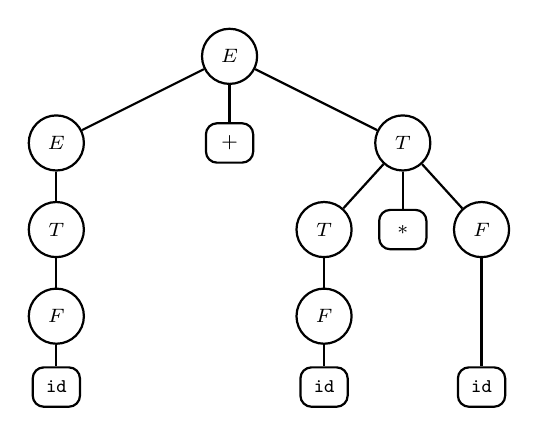
\begin{tikzpicture}[
    every node/.style={font=\scriptsize},
    nt/.style={draw, circle, thick, minimum size=7mm},
    t/.style={draw, rounded corners, thick, minimum width=6mm, minimum height=5mm}
]
    \node<2->[nt] (E0) at (0,0) {$E$};

    \node<3->[nt] (E1) at (-2.2,-1.1) {$E$};
    \node<3->[t]  (plus) at (0,-1.1) {$+$};
    \node<3->[nt] (T1) at (2.2,-1.1) {$T$};

    \draw<3->[thick] (E0) -- (E1);
    \draw<3->[thick] (E0) -- (plus);
    \draw<3->[thick] (E0) -- (T1);

    \node<4->[nt] (Tleft) at (-2.2,-2.2) {$T$};
    \node<4->[nt] (T2) at (1.2,-2.2) {$T$};
    \node<4->[t]  (times) at (2.2,-2.2) {$*$};
    \node<4->[nt] (F3) at (3.2,-2.2) {$F$};

    \draw<4->[thick] (E1) -- (Tleft);
    \draw<4->[thick] (T1) -- (T2);
    \draw<4->[thick] (T1) -- (times);
    \draw<4->[thick] (T1) -- (F3);

    \node<5->[nt] (Fleft) at (-2.2,-3.3) {$F$};
    \node<5->[nt] (F2) at (1.2,-3.3) {$F$};

    \draw<5->[thick] (Tleft) -- (Fleft);
    \draw<5->[thick] (T2) -- (F2);

    \node<6->[t] (a1) at (-2.2,-4.2) {$\mathtt{id}$};
    \node<6->[t] (a2) at (1.2,-4.2) {$\mathtt{id}$};
    \node<6->[t] (a3) at (3.2,-4.2) {$\mathtt{id}$};

    \draw<6->[thick] (Fleft) -- (a1);
    \draw<6->[thick] (F2) -- (a2);
    \draw<6->[thick] (F3) -- (a3);
\end{tikzpicture}
